\chapter {Ferramentas de Análise Estática}

Projetar analisador estático que verifique o código desenvolvido não é uma simples tarefa, entretanto com a infraestrutura provida pelo EclipseJDT~\cite{EclipseJDT} tornou menos árduo esta jornada possibilitando projetar uma arquitetura para este analisador onde o desenvolvedor concentre-se apenas na produção de seus \textit{Visitors}. 

Um ponto de estrema relevância foi tornar este analisador independente de qualquer plataforma e \acs{IDE} foi um ponto vital para o desenvolvimento deste projeto que não tem como intuito ser plugin de qualquer \acs{IDE} o que acarretaria na limitação do seu uso a um cenário específico. Utilizando a portabilidade nativa entre as plataformas provido pela linguagem Java este trablho foi concebido com intuíto de atender ao mais diversos desenvolvedores quer utilizem linux, windows, mac ou qualquer outro sistema operacional que tenha suporte para Java.

A análise tem como início a seleção de projetos, nesse caso seleção em repositórios públicos, onde após o download é informado analisador o diretório raíz onde estes estão localizados. Após é iniciado uma listagem dos arquivos fonte Java contidos nos projeto e contabilizados o total de \acs{LOC} e criado uma árvore sintática para cada arquivo encontrado através de um \textit{parser} provido pela biblioteca EclipseJDT~\cite{EclipseJDT}. Em seguida os \textit{Visitors} são instanciados com o objetivo de percorrer os nós destas árvores para pesquisar por contruções de código previamente determinadas.

Todas as contruções pesquisadas quando encontradas pelos \textit{Visitors} são armazenadas temporariamente enquanto o analisador verifica todo projeto, quando é verificado a última árvore sintática pelos \textit{Visitors} é iniciado o processo de exportar os dados encontrados para um arquivo \acs{CSV} o conteúdo relevate destes blocos, a Figura:~\ref{fig:Arquitetura} demostra de maneira clara o funcionamento do analisador. Após a exportação dos dados o analisador inicia todo processo novamente caso exista mais de um projeto.

Devido ao mescanismo de \textit{reflection} proveniente da linguagem Java, o desenvolvedor não tem a necessidade de implementar código para exportação de dados tendo em vista que isto ocorre automaticamente através da introspecção realizada pelo analisador extraíndo os dados armazendados pelos \textit{Visitors}.

	\begin{figure}[h]
		\center
		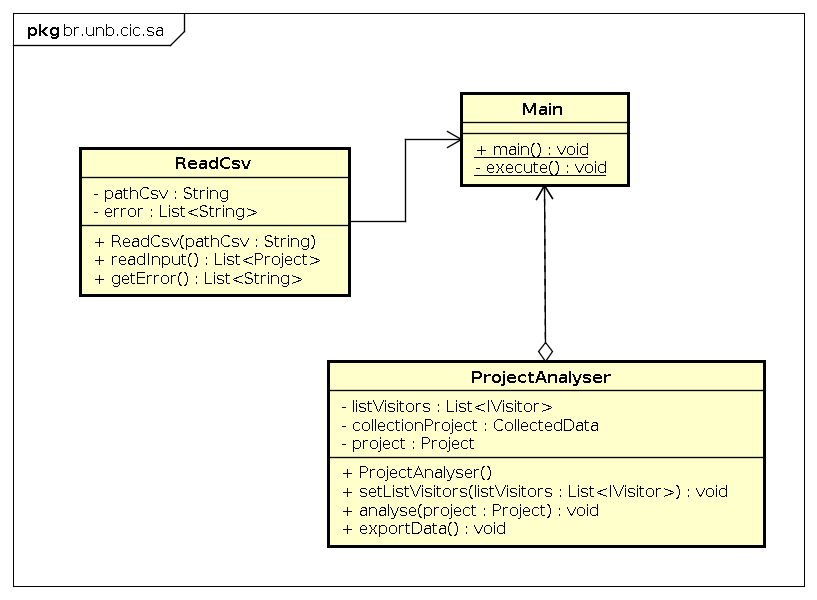
\includegraphics[scale=0.52]{Imagens/Arquitetura}
		\label{fig:Arquitetura}
		\caption{Funcionamento analisador estático.}
	\end{figure}


\section{Arquitetura}

\subsection{Visitors}

\begin{table}[ht!] \footnotesize
	\centering
	\caption{Tabela de Visitors criados com suas respectivas atribuições}
	\label{tab:VisitorsCriados}	
    \begin{tabular}{ >{\arraybackslash}p{2.2in} | >{\arraybackslash}m{3.8in} }
%		\begin{tabular}{M|p{9cm}}% centered column
			\hline 
			\textbf{Visitor} & \textbf{Atribuição}\\ \hline \hline
			
			AICVisitor & Pesquisar \textit{Anonymous Inncer Class} declaradas.\\ \hline
			
			EnumDeclarationVisitor 	& Pesquisa por \textit{Enums} declarados.\\ \hline
			
			ExistPatternVisitor	& Pesquisa \textit{EnhancedFor} que iteram sobre uma coleção procurando qualquer ocorrência nessa coleção.\\ \hline
			
			FieldAndVariableDeclarationVisitor & Lista todos as variáveis declaradas como os respectivos tipos.\\ \hline
			
			FilterPatternVisitor &  Lista todos os \textit{EnhancedFor} que iteram uma coleção filtrando elementos desta mesma coleção.\\ \hline
			
			ImportDeclarationVisitor & Lista todos os \textit{imports}.\\ \hline
			
			LambdaExpressionVisitor & Pesquisa casos de utilização da expressões lambda. \\ \hline
			
			LockVisitor & Verifica se nos métodos declarados existe alguma variável chamada Lock, ReentrantLock, ReadLock ou WriteLock. \\ \hline
			
			MapPatternVisitor & Pesquisa \textit{EnhancedFor} que iteram sobre uma coleção onde seja aplicado algum método sobre os items desta coleção. \\ \hline
			
			MethodCallVisitor & Verifica onde esta sendo utilizado reflection no projeto.\\ \hline
			
			MethodDeclarationVisitor & Coleta informações sobre os métodos declarados nos projetos. \\ \hline
			
			ScriptingEngineVisitor & Verifica se o projeto faz chamada a algum \textit{Scripting}.\\ \hline
			
			SwitchStatementVisitor & Pesquisa \textit{Switchs} que utlizam \textit{String} como parâmetro.\\ \hline
			
			SwitchStringOpportunitiesVisitor &  Pesquisa \textit{If-Else} aninhados onde no \textit{If} contenha \textit{String}, caracterizando uma possibilidade de adoção de \textit{Switch} com \textit{String}.\\ \hline
			
			
			TryStatementVisitor & Pesquisa \textit{trys} que utilizar \textit{resource}, adoção de \textit{multicatch} e \textit{trys} que possuem \textit{catchs} aninhados.\\ \hline
			
			TypeDeclarationVisitor & Pesquisa todos os tipos declarados.\\ \hline 		
		\end{tabular}
\end{table}


Conforme mencioando anteriormente, nos \textit{Visitors} é onde deve ser concentrado todo esforço para extair as informações com a maior confiabilidade possível. Efetuar a criação de novos \textit{Visitor} quando necessário na atual arquitetura deste analisador requer que todos sejam  obrigatoriamente extendidos da classe \textit{Visitor.java} a qual por sua vez extende da \acs{API}  \textit{ASTVisitor}, e implementa uma interface parametrizada que possui um coleção do tipo, \textit{\textbf{<T>}}, onde esta terá a responsabilidade de armazenar os dados minerados pelos \textit{Visitors}. 

Os \textit{Visitors} criados necessitam somente que cada \textit{Visitor} sobrescreva o método \textit{public boolean visit} que é um método abstrato da classe \textit{ASTVisitor} de acordo com sua necessidade.

\begin{lstlisting}
package br.unb.cic.sa.visitors;

import org.eclipse.jdt.core.dom.ASTVisitor;
import org.eclipse.jdt.core.dom.CompilationUnit;
import br.unb.cic.sa.model.Data;

public class Visitor<T> extends ASTVisitor implements IVisitor<T> {
	protected CompilationUnit unit;
	protected Data<T> collectedData;
	protected String file;
	
	public Visitor() {}
	
	@Override
	public void setUnit(CompilationUnit unit) { this.unit = unit; }
	
	@Override
	public void setCollectedData(Data<T> colletion) { this.collectedData = colletion; }
	
	@Override
	public void setFile(String file) {	this.file = file; }

	@Override
	public Data<T> getCollectedData() {	return collectedData;	}	
}
\end{lstlisting}


A tabela:~\ref{tab:VisitorsCriados} detalha os 17 \textit{Visitors} criados com a respectiva descrição do trabalho ralizado. Como forma de exemplificar a criação de um \textit{Visitors}, etapa a qual é composta de 4 passos quo serão demonstrados a seguir.

A investigação para saber como o tratamento de exceção Java tem sido utilizado acarretou na criação de um \textit{Visitor} específico para este fim, \textit{TryStatementVisitor}, responsável por pesquisar este mecanismo o qual pode contar com alguma evoluções ao logo do histórico da linguagem Java. A pesquisa é iniciada encontrando blocos \textit{trys/catch}, onde destes será coletadas as infomações referentes a adoção de \textit{resources} e oportunidade de utilizar \textit{multicatch} em blocos \textit{trys} que contenham \textit{catchs} iguais ainhados.
%, neste caso de oportunidades os \textit{catchs} são testados por igualdade mas é trivial a utilização de um algoritmo mais avançado que teste a similaridade.

Criaçãd do \textit{Visitor TryStatementVisitor} com exemplo.

	\begin{enumerate}
		\item Inicialmente é necessário criar a classe modelo onde esta terá atribuição de receber os dados que serão extraídos pelos \textit{Visitors}, basicamente as classes modelos são compostas de \textit{getters} e \textit{setters} e são declaradas no pacote  \textit{\textbf{br.unb.cic.sa.model}}.
			\begin{lstlisting}
package br.unb.cic.sa.model;

public class TryStatementData  {
	private String file;
	private int startLine;
	private int endLine;
	private boolean tryWithResource = false;
	private boolean multiCatch = false;
	
	public TryStatementData(String file, int startLine, int endLine){
		this.file = file;
		this.startLine = startLine;
		this.endLine = endLine;
	}
	
	//getters and setters
}
			\end{lstlisting}
			
			
		\item Em seguida, é concebida a criação do \textit{Visitor} no pacote \textit{\textbf{br.unb.cic.sa.visitors}} onde esta nova classe será extendida da classe parametrizada \textit{\textbf{Visitor<TryStatementData>}} apresentada anteriormente onde a parametrização desta classe é o modelo criado anteriormente.
			
			\begin{lstlisting}
package br.unb.cic.sa.visitors;

import java.util.List;
import org.eclipse.jdt.core.dom.CatchClause;
import org.eclipse.jdt.core.dom.TryStatement;
import br.unb.cic.sa.model.TryStatementData;
import br.unb.cic.sa.similarity.BasicSimilarityChecker;
import br.unb.cic.sa.similarity.SimilarityChecker;

public class TryStatementVisitor extends Visitor<TryStatementData> {

	SimilarityChecker similarity;

	public TryStatementVisitor() {
		similarity = new BasicSimilarityChecker();
	}

	@Override
	public boolean visit(s node) {

		TryStatementData t = new TryStatementData(this.file, unit.getLineNumber(node.getStartPosition()),
				unit.getLineNumber(node.getStartPosition() + node.getLength()));
		
		if (node.resources().size() > 0) {
			t.setTryWithResource(true);
		}
	
		if (node.catchClauses().size() > 1) {
			if (this.checkSimilarity(node.catchClauses())) {
				t.setMultiCatch(true);
			}
		}

		this.collectedData.addValue(t);

		return super.visit(node);
	}
	
	private boolean checkSimilarity(List<CatchClause> catchClause) {
		for (CatchClause cc : catchClause) {
			for (CatchClause cn : catchClause) {
				// To ignore the same catch in loops
				if (!cc.equals(cn)) {
				
				//Chamada externa para testar similaridade
					if (this.similarity.checkSimilarity(cc.getBody(),
														cn.getBody())) {
						return true;
					}
				}
			}
		}
		return false;
	}

}
			\end{lstlisting}
			
		 Na linha24, é testada a condição para saber se este bloco fez adoção de \textit{Resouce}. Na linha 30 é verificado que o bloco é um possível caso de \textit{multicatch} pois existe mais de um bloco. Na linha 39 tem-se o método \textit{checkSimilarity} o qual efetua a comparação dos blocos \textit{Catch} aninhados em um \textit{try}, entretando de forma trivial na linha 46, pode ser utilizado um algoritmo mais sofisticado para testar sim a similaridade modeificando apenas o método \textbf{\textit{checkSimilarity}} da classe \textit{\textbf{SimilarityChecker}} o que não resulta em mudanças neste \textit{Visitor}.
		
	
			\item Em seguida deve-se declarar o cabeçalho no arquivo \textit{resource/Beans.xml} do \textit{Spring} que estará presente no \acs{CSV} de saída. Onde este cabeçalho é composto pelo dados que serão extraídos pelos \textit{Visitors} e armazenados no modelo criado.
			
			\begin{lstlisting}
<bean id="tryStatementData" class="br.unb.cic.sa.model.CSVData">
	<property name="outDir" value="output"/>
	<property name="fileName" value="tryStatement"/>
	<property name="head" value="typeProject, before, project, version, file, start, end, resource, multiCatch"/> 
</bean>
			\end{lstlisting}
			
			
			\item Por fim declarar o \textit{Visitor} como um \textit{bean} do \textit{Spring} para que este seja injetado no projeto e assim realize sua pesquisa.
			
			\begin{lstlisting}
<bean id="tryStatementVisitor" class="br.unb.cic.sa.visitors.TryStatementVisitor">
	<property name="collectedData" ref="tryStatementData"/>
</bean>
			\end{lstlisting}
			
	\end{enumerate}




\subsection{Dados Coletados}


%O Eclipse Java {\it development tools} (JDT), fornece plugins que implementam a IDE eclipse servindo com apoio para o desenvolvimento de qualquer aplicativo Java, inclusive plugins para a própria IDE Eclipse. São cinco os componentes que compõem o JDT, e cada componente pode operar com um projeto independente, que são:

%	\begin{itemize}
%		\item \textbf{APT} fornece plugins que adicionam e fornecem suporte ao processamento de anotações java.
%		\item \textbf{Core} é o core da infraestrutura Java da IDE eclipse provendo compiladores, API's modelos definidas em árvores Java, documentação, assitente de código, suporte e formatação de código fonte.
%		\item \textbf{Debug} componente de depuração da plataforma sendo definido independente da linguagem utilizada.
%		\item \textbf{Text} fornece blocos básicos para editores de texto e textos dentro do eclipse e ainda contribui com o editor de texto padrão do eclipse. \item \textbf{UI} prove toda interface que necessite de iteração com o usuário final, e ainda fornece a manipulação e visualização do código Java na IDE.
%	\end{itemize} 
%	

%\section {Arquitetura}
%A arquitetura do analisador exibido na Figura: \ref{fig:arqGeral} foi implementado utilizando como base os componentes \acs{JDT} porém de maneira independente de qualquer \acs{IDE} neste caso o Eclipse e não a intenção de criar um {\it plugin} para \acs{IDE} mas sim uma ferramenta que pode ser utilizada com auxílio ao longo do processo de desenvolvimento ou para minerar dados sobre evolução do software identificando contruções ultrapassadas.
%
%\begin{figure}[h]
%	\center
%	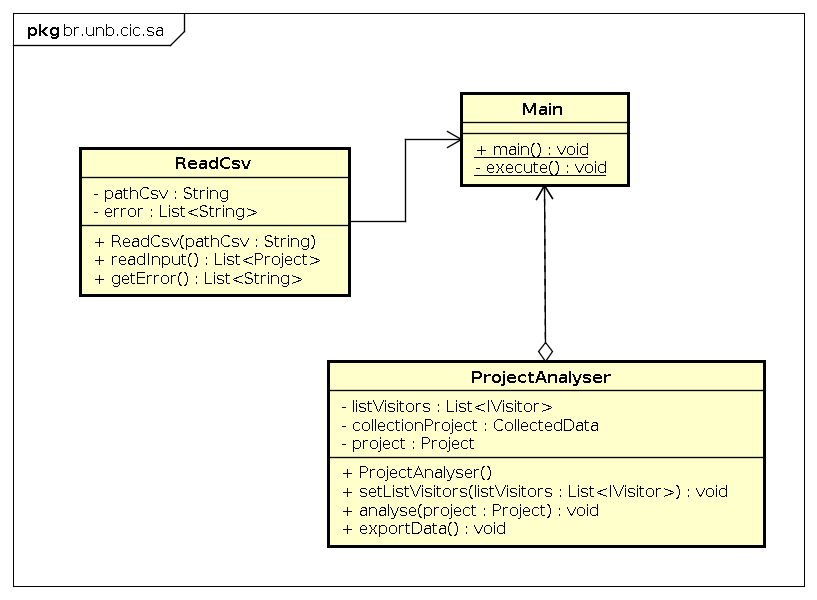
\includegraphics[scale=0.45]{Imagens/Arquitetura}
%	\label{fig:arqGeral}
%	\caption{Arquitetura geral do software.}
%\end{figure}
%
%
%Este analisador tem com base para seu funcionamento o uso de {\it visitors} \cite{Gamma:1995} exemplificado na Figura: \ref{fig:arqVisitor} os quais possuem inteligência para identificar padrões de código que podem vir a ser especificados pelo desenvolvedor. A pesquisa pela adoção de códigos recentemente adicionados a novas {\it releases} da linguagem Java como {\it multicatchs} e podem até mesmo efetuar a pesquisa de código ultrapassados através destes padrões para que possam vir a sofrer um \textit{refactoring} caso o desenvolvedor assim que julgue necessário conforme é o caso de vários {\it catchs} aninhados que pode ser um potencial caso de se tornar um bloco único de {\it multicatch} tornando o código mais elegante, atual e legível.
%
%Para exemplificar um padrão de pesquisa de um visitor segue o código abaixo como trecho do visitor que pesquisa por \textit{try's} que contém mais de um \textit{catch} aninhado onde este podem ser migrados para um único bloco \textit{multicatch}. 
%\begin{lstlisting}
%if (node.catchClauses().size() > 1){
%	if(this.checkSimilarity(node.catchClauses()){
%		...
%	}
%}
%\end{lstlisting}

%Tais analisador tem como entradas válidas um único arquivo arquivo separado por vírgula (CSV) que possui em seus campos o nome dos projeto, versões e caminho para que cada um seja analisado. Após o {\it input} é realizado uma pesquisa em seu diretório \textit{src} o qual contém os códigos Java que compõem o projeto, após todos os arquivos listas é realizado um parse para a construção de árvores de sintáxe abstratas (AST) uma por arquivo e dai é lançando os {\it visitors}  \cite{Gamma:1995:DPE:186897} com suas respectivas inteligências para pesquisar os padrões previamente definidos os quais são armazenados em uma única coleção de dados que gera um CSV para cada padrão designado e dentro informando onde e em qual versão do projeto fora encontrado.\\

%\subsection{Visitors}
%\begin{figure}[h]
%\center
%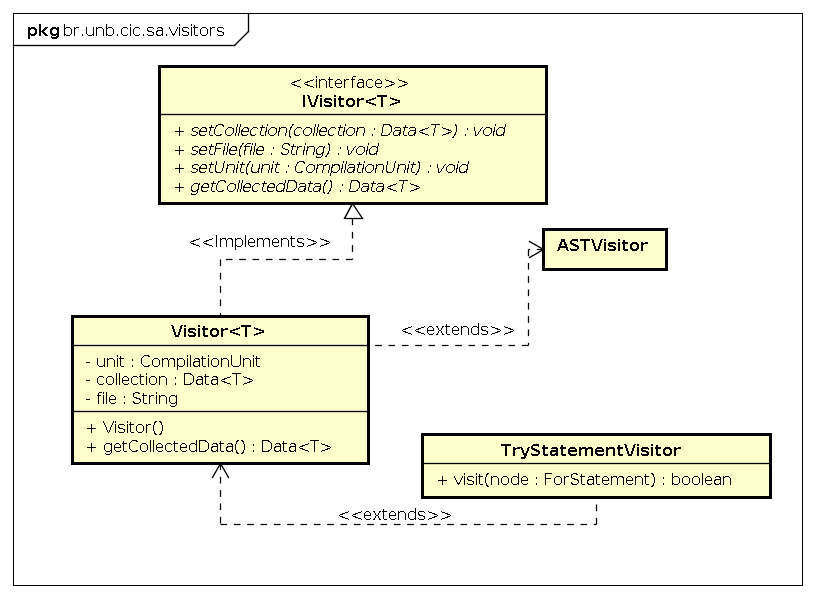
\includegraphics[scale=0.5]{Imagens/Visitors}
%\label{fig:arqVisitor}
%\caption{Organização dos Visitors.}
%\end{figure}
%
%Para a implementação de um \textit{visitor} é necessário extender da classe parametrizada \textit{Visitor<T>.java} onde \textit{T} é apenas um modelo que armazena dados como o arquivo onde foi encontrado a construção conforme exibido na Figura:~\ref{fig:ProjectAnalyser}, linha de código inicial e final do bloco. A classe \textit{Visitor<T>} implementa um interface parametrizada, \textit{Data<T>}, que por sua vez é a coleção de dados os quais foram pesquisados pelos \textit{visitors}. Segue um simples exemplo de como implementar um \textit{visitor}. 
%
%\begin{lstlisting}
%public class MeuVisitor extends Visitor<LambdaModel>{
%	public boolen visit(Statement node){
%		.....
%		return super.visit(node);
%	}
%}
%\end{lstlisting}
%
%Após a implementação de \textit{visitor} desejado, é necessário declarar o \textit{visitor} no \textit{Beans.xml} com seu respectivo cabeçalho para que este seja injetado na classe \textit{ProjectAnalyser.java} para que a pesquisa ao qual foi condicionado nas árvores sintátitcas dos códigos fontes do projetos geradas pela classe \textit{Parser.java} seja realizada com sucesso. Abaixo é exemplificado o cabeçalho do arquivo \acs{CSV} de saída e a declaração do Visitor no \textit{Beans.xml}.
%
%\begin{lstlisting}
%	// Visitor com o respectivo cabecalho 
%	<bean id="tryStatementData" class="br.unb.cic.sa.model.CSVData">
%		<property name="outDir" value="output"/>
%		<property name="fileName" value="tryStatement"/>
%		<property name="head" value="typeProject, before, project, version, file, start, end, resource, multiCatch"/> 
%	</bean>
%	...
%	
%	// Visitor com sua respectiva Data<T> collection
%	<bean id="tryStatementVisitor" class="br.unb.cic.sa.visitors.TryStatementVisitor">
%		<property name="collectedData" ref="tryStatementData"/>
%	</bean>
%	...
%	
%	//Lista de visitors a ser injetada na Classe ProjectAnalyser.java
%	<bean id="pa" class="br.unb.cic.sa.ProjectAnalyser">
%		<property name="listVisitors">
%		 	<list>	
%		 		<ref bean="tryStatementVisitor"/> 
%		 	</list>
%		</property>
%	</bean>
%		
%\end{lstlisting}
%







% vale resaltar que a classe \textit{Visitor.java} extende por sua vez de ASTVisitor a qual é fornecida pelo Core do JDT eclipse tendo como método principal utilizado neste projeto o \textbf{{\it boolean visit(Statement node)}} o qual recebe como parâmento qualquer {\it Statement} descrito na lib JDT, este método é sobrescrito com todo conteúdo necessário para recolher as métricas de acordo com os padrões previamente estabelecidos.\\
%\clearpage
%\begin{figure}[h]
%	\center
%	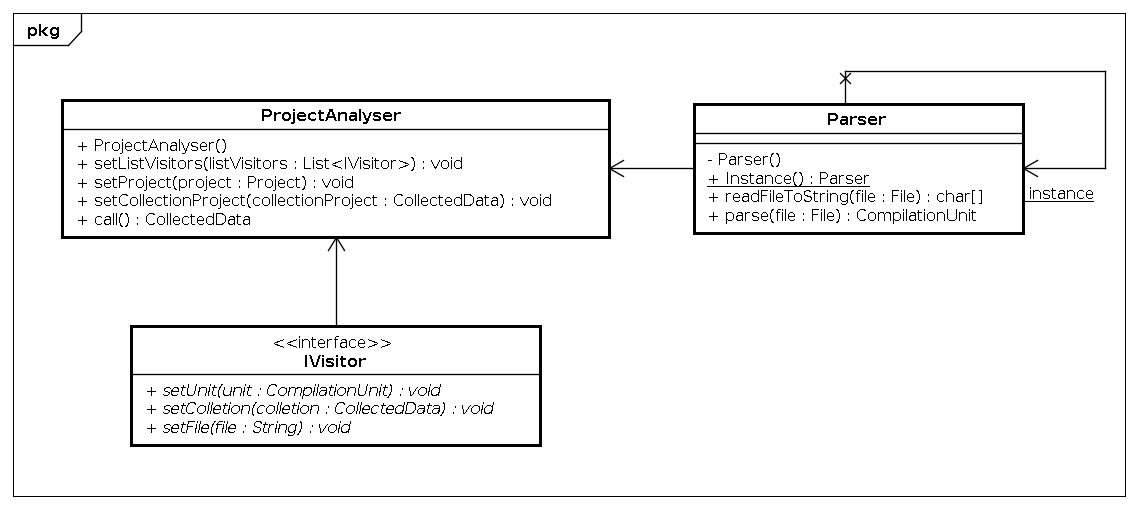
\includegraphics[scale=0.4]{Imagens/ProjectAnalyser}
%	\label{fig:ProjectAnalyser}
%	\caption{Project analyser.}
%\end{figure}


%Para exportar os dados para o arquivo \acs{CSV} é utlizado \textit{reflection} onde é verificado todos os valores \textit{T} armazenados pelos \textit{Visitors} e extratido dos métodos \textit{get} contidos nos modelos os quais foram criados para armazenar os dados pesquisados nas árvores sintáticas. Esta característica do analisador permite que o usuário não se preocupe com a exportação dos dados que é feita de forma automática, concentrando apenas seus esforços na criação dos \textit{Visitors}.

%Este diagrama exibe o coração da aplicação pois é aqui que ocorre a transformação de todo código Java que compõe o projete em árvore sintática para que os {\it visitors}  \cite{Gamma:1995:DPE:186897} possam pesquisar em seus nós pelos padrões estabelecidos.\\

%Um ponto interessante é que o \textit{ProjectAnalyser.java} Figura: ~\ref{fig:ProjectAnalyser} não tem a responsabilidade de instanciar a lista de IVisitor a qual possui referência pois estas são injetadas usando o padrão de projeto injeção de dependência\textbf{(DI)} o qual aqui faz-se presente através do {\it framework spring} que injeta uma lista de \textit{bean} onde cada \textit{bean} representa cada classe de extendida de {\it Visitor} descrita anteriormente.\\



%\subsection{Injeção de Dependência}
%
%O padrão de projeto inversão de controle \textbf{(IoC)} e injeção de dependência \textbf{(DI)} é utilizado quando deseja-se obter um baixo nível de acoplamento entre módulos que compõem um sistema tornando mais suave ou até mesmo removendo o acoplamento entres módulos para que seja mais fácil evoluir e manter o software. Desta forma a injeção faz-se de maneira configurável através de um arquivo \textit{XML} ou até mesmo uma classe \textit{Java}. Para tal função usaremos o {\it framework Spring} devido sua consolidação e popularidade no assunto.
%
%Para preparar o ambiente de acordo com as especificações do {\it Spring} é necessário definir o contexto da aplicação e para isso é faz-se necessário criar antes de injetar as dependências as configurações iniciais. Dentre as possíveis formas disponibilizadas pelo {\it framework} de conceder tal configuração para criação um contexto para aplicação \textit{ApplicationContext} o projeto segue com a criação de um arquivo \textit{XML} o que concentra as referências necessárias de quais objetos e onde estes serão injetados. O arquivo \textit{XML} criado para tal finalidade é o \textit{'Beans.xml'} . Atualmente na versão 4.1.6 do {\it framework spring} é possível utilizar uma classe para fazer o mesmo trabalho do arquivo \textit{XML}. 
%
%%Configuração necessária para o funcionamento da injeção de dependências com {\it Spring} conforme explicado na documentação do {\it framework} conforme \cite{SPRING_REF}.\\
%%\begin{lstlisting}
%%<?xml version="1.0" encoding="UTF-8"?>
%%	<beans xmlns="http://www.springframework.org/schema/beans"
%%		xmlns:xsi="http://www.w3.org/2001/XMLSchema-instance" xmlns:context="http://www.springframework.org/schema/context"
%%		xsi:schemaLocation="http://www.springframework.org/schema/beans 
%%		http://www.springframework.org/schema/beans/spring-beans-3.0.xsd
%%		http://www.springframework.org/schema/context 
%%		http://www.springframework.org/schema/context/spring-context-3.0.xsd">
%%
%%		<bean id="tsVisitor" class="br.unb.cic.sa.visitors.TryStatementVisitor"/>
%%		<bean id="opportinitiesLambda" class="br.unb.cic.sa.visitors.OpportunitiesLambdaVisitor"/>
%%		<bean id="opportinitiesSwitchString" class="br.unb.cic.sa.visitors.OpportinitiesSwitchString"/>
%%	</beans>
%%	
%%	<bean id="pa" class="br.unb.cic.sa.ProjectAnalyser">
%%		<property name="listVisitors">
%%		<list>
%%			<ref bean="tsVisitor"/>
%%			<ref bean="opportinitiesLambda"/>
%%			<ref bean="opportinitiesSwitchString"/>
%%		</list>
%%		</property>
%%	</bean>
%%\end{lstlisting}
%
%
%O {\it framework} trabalha com \textit{beans} onde cada \textit{bean} representa uma classe Java a ser injetada vale ressaltar que essas por simplicidade devem ter o construtor sem parâmetros para que o trabalho possa ocorrer da maneira mais simples, caso seja necessário parâmetros estes sejam passados vias os métodos Sets.
%
%Identificação de cada bean no arquivo de configuração \textit{XML}, é atributo \textbf{id} contido na {\it tag} \textbf{bean} onde cada deve ser único para que a gerência das dependências ocorra da forma preconizada pelo {\it framework}.
%
%Todos os {\it Beans} são injetados na classe \textit{ProjectAnalyser.java} através de uma lista de IVisitor. E desta forma indicamos no \textit{XML} através da tag \textbf{<property name="listVisitors">} onde o atributo \textbf{name} deve conter o mesmo nome que o atributo na classe Java,  neste caso o algo é \textbf{listVisitors} que existe uma lista de IVisitor com este mesmo nome dentro da classe \textit{ProjectAnalyser.java}.
%
%Para concluir com sucesso a injeção faz-se necessário somente indicar em qual classe e em qual local será injetada tal dependêcia, nesse caso a classe é a \textit{ProjectAnalyser.java} e o local é definido pela anotação \textbf{\textit{@Autowired}} logo acima do atributo o qual será injetado.
%
%\begin{lstlisting}
%	public class ProjectAnalyser... {
%
%		@Autowired
%		private List<IVisitor> listVisitors;
%		.
%		.
%		.
%	}
%\end{lstlisting}
%
%Para finalizar todo ambiente de configuração de injeção de dependência é necessário somente criar uma classe que seja um {\it Singleton} \cite{Gamma:1995} conforme cita Gamma e amigos e faz-se necessária conforme indica a documentação \cite{SPRING_REF}, para ter o controle de que exista somente um único ambiente de injeção. Tal padrão que controla a quantidade de instâncias dos objetos se faz presente através da classe \textit{CDI.java}.
%\begin{lstlisting}
%	public class CDI {
%		private static CDI instance;
%		private ApplicationContext ctx;
%		
%		private CDI(){ 
%			ctx = new ClassPathXmlApplicationContext("Beans.xml");
%		}
%		
%		public static CDI Instance(){
%			if(instance == null)
%				instance = new CDI();
%		
%			return instance;
%		}
%		
%		public ApplicationContext getContextCdi(){
%			return ctx;
%		}
%	}
%\end{lstlisting}
%
%Abaixo segue bibliotecas necessárias para que o ambiente de injeção de dependência utilizando o textit{spring framework} \cite{SPRING_REF} ocorra de maneira correta na linguagem \textit{Java}, estas devem ser adicionada como dependências do Maven.


%\subsection{Apache Maven}
%Afim de gerenciar \textit{builds} deste analisador estático, o Maven foi introduzido para tornar as configurações uniformes no ambiente de desenvolvimento deste seguindo as boas práticas, compilação, gerência de dependências e distribuição da aplicação, a tabela \ref{tab:DependenciasMaven} detalhas as bibliotecas e versões utilizadas.

%O arquivo pom.xml segundo a documentação \cite{docMaven}, \textit{project object model} é a essência de um projeto Maven, com poucas configurações é possível gerências as dependências, centralizando documentação do projeto e a compilação de \textit{builds} para a distribuição da aplicação (por exemplo, \textit{.jar, .war ou .ear}).\\


%\begin{table}[ht]
%	\centering
%	\caption{Dependências gerenciadas através do Maven}
%		\label{tab:DependenciasMaven}
%		\begin{tabular}{c|c}% centered column
%			\hline \hline
%			\textbf{Dependência}    &   \textbf{Versão}\\ \hline
%			junit 			    	&	4.12 \\ \hline
%			commons-collections 	&	3.2.1 \\ \hline
%			commons-configuration 	&	1.6 \\ \hline
%			commons-lang 	    	&	2.5 \\ \hline
%			ommons-logging 			&	1.1.1 \\ \hline
%			org.eclipse.core.contenttype & 3.4.100.v20100505-1235 \\ \hline
%			org.eclipse.core.jobs 		&	3.5.100.v20110404 \\ \hline
%			org.eclipse.core.resources  &	3.7.100.v20110510-0712 \\ \hline
%			org.eclipse.core.runtime		&	3.1.200-v20070502 \\ \hline
%			org.eclipse.equinox.common		&	3.6.0.v20100503 \\ \hline
%			org.eclipse.equinox.preferences &	3.4.0.v20110502 \\ \hline
%			org.eclipse.jdt.core 			&	3.10.0.v20140604-1726 \\ \hline
%			org.eclipse.osgi 	&	3.7.1 \\ \hline
%			org.osgi.core 		&	6.0.0 \\ \hline
%			spring-aop 	    	&	4.1.6.RELEASE \\ \hline
%			spring-beans 		&	4.1.6.RELEASE \\ \hline
%			spring-context 		&	4.1.6.RELEASE \\ \hline
%			spring-context 		&	4.1.6.RELEASE \\ \hline 		
%			spring-expression 	&	4.1.6.RELEASE \\ \hline
%		\end{tabular}
%	
%\end{table}



